\documentclass[conference]{IEEEtran}
% \IEEEoverridecommandlockouts
% The preceding line is only needed to identify funding in the first footnote. If that is unneeded, please comment it out.
\usepackage{cite}
\usepackage{amsmath,amssymb,amsfonts}
\usepackage{algorithmic}
\usepackage{graphicx}
\usepackage{textcomp}
\usepackage{xcolor}
\usepackage{hyperref}
\usepackage{subfig}
\usepackage[font=scriptsize]{caption}
\setlength{\belowcaptionskip}{-10pt}
\def\BibTeX{{\rm B\kern-.05em{\sc i\kern-.025em b}\kern-.08em
    T\kern-.1667em\lower.7ex\hbox{E}\kern-.125emX}}

\newcommand\ci{\perp\!\!\!\perp}

\begin{document}

\title{Graph Structure Learning for Traffic Flow} 
\author{\IEEEauthorblockN{Clara Cousins\\\href{mailto:ccousins@college.harvard.edu}{ccousins@college.harvard.edu}}
\\[-9.0ex]
\and
\IEEEauthorblockN{William Drew\\\href{mailto:wdrew@college.harvard.edu}{wdrew@college.harvard.edu}}
\\[-9.0ex]
}
\maketitle
\begin{abstract}
Competing content delivery services may not have access to packet-level information at each others' servers, but would benefit from understanding traffic flow in networks they use. We propose a novel, noninvasive solution to identify traffic flow using only packet counts at internet service provider routers with graphical structure learning. We used simulated data in multiple topologies and identified the fast incremental association Markov blanket algorithm for a directed acyclic graph (DAG) as an appropriate structure learning algorithm. For networks with tree and mesh components, this algorithm found the ratio of true found edges to real edges was 0.76, while the ratio of false found edges to total found edges was 0.39, indicating that DAG learning may be suitable for revealing network-wide traffic.

\end{abstract}

\begin{IEEEkeywords}
topology, traffic, graph, structure learning 
\end{IEEEkeywords}

\section{Introduction}
With an increasing reliance on internet networks to deliver content to consumers, there is a growing need for businesses to understand network-wide traffic. However, due to the sensitivity of network traffic information including port number, protocol type, and packet routing path, there is a particular challenge in recovering network traffic flows from information that is not embedded in the packets themselves. A noninvasive network analysis method (i.e., not requiring packet inspection nor the routing paths) would be revolutionary to the field. In this work, we explore how undirected graphical models (UGMs) and directed acyclic graphs (DAGs) can model network-wide traffic based on packet counts at routers.

\section{Problem to Solve}

To what extent does UGM and DAG structure learning reveal network traffic flows based on packet counts at internet service provider (ISP) routers?

\section{Background, Motivations, and Prior Work}

Content delivery services, such as Netflix and Hulu, compete for consumers but may not have access to packet-level information at each other's routers or servers. Netflix and Hulu would be motivated to compare their traffic flow patterns among a collection of routers (such as for a certain ISP in the metro Boston area) in order to identify the routers that are bottlenecks for their own or their competitor's traffic as well as the regions each company reaches effectively. This could enable content service providers to craft new subscriber services, optimize shared resource utilization, and understand the limitations of the content delivery network \cite{b1}.

Traffic flow may be understood at various degrees of granularity, including the packet (i.e., reading IP header with Cisco NetFlow \cite{b2}), individual host (i.e., probing connectivity with dummy packets from a given host \cite{b3}), or aggregate host (i.e, traffic dispersion graphs drawn from routing paths \cite{b1}) level. Artificial \cite{b4} and graphical \cite{b5} neural networks are also emerging as approaches to model network-wide traffic flows.

\section{Project Goals \& Evaluation Metric}

The goal of this project is to determine which UGM or DAG structure learning algorithms can reveal accurate traffic flow topologies using simulated networks adhering to a link state routing scheme with Dijkstra's shortest path algorithm. This goal would be successfully achieved if we can find algorithms such that
\[
\frac{\text{True found edges}}{\text{Total real edges}} > \frac{\text{False found edges}}{\text{Total found edges}}
\]
A well-performing algorithm should have a high proportion of true found edges to total true edges (TFT) indicating that the algorithm discovered many edges in the original topology and a low proportion of false found edges to total found edges (FFF) indicating that the algorithm found few extraneous edges.

\section{Proposed Approach}

We propose a novel method to learn aggregate flows across hosts using only packet counts at ISP routers. Critically, this approach noninvasively learns network traffic flows without examining sensitive fields such as destination IP addresses, port numbers, protocol types, nor packet routing paths. We accomplish this using UGM and DAG structure learning algorithms to predict network topologies.

\section{Intellectual Points}

Both UGMs and DAGs encode the joint probability distribution of a collection of random variables (``nodes”) with conditional dependencies (``edges") indicated. Whereas DAGs have directed edges that can be interpreted as causal effects, UGMs have all bidirectional edges and therefore may contain cycles. An edge in a UGM effectively represents where conditional independence between two nodes does not exist given its neighboring nodes in the graph. Conditional independence exists between random variables $X$ and $Y$ given $Z$ with nonzero probability $\left(X \ci Y | Z \right)$ if $P(X \ci Y | Z) = P(X | Z) * P(Y | Z)$ where $P(A | B) = P(A, B) / P(B)$. An edge in a DAG from a parent (direct ancestor) to child (direct descendant) node exists where the values in the child are conditionally independent of the other nodes in the DAG (save the children's own descendants) given the values of the parents.

DAGs rely on certain assumptions to allow directed edges to indicate causal effects between nodes. These include the causal Markov condition, faithfulness, and causal sufficiency \cite{b6}. Briefly, the causal Markov condition states that a node is conditionally independent of all other nodes except for its children given its parents \cite{b7}. Faithfulness means that the DAG learned from the data contains conditional dependencies that are indeed reflected in the data and are not the result of model parameters cancelling each other during the learning process \cite{b8}. Finally, causal sufficiency ensures that enough nodes are included in the DAG such that the conditional dependencies learned have the potential to reflect real causal effects without hidden nodes being responsible for the relations \cite{b8}.

There are three main classes of algorithms used to learn UGM and DAG structures from observational data (i.e., without manipulation of the values at any node). Briefly, score-based approaches (such as greedy hill-climbing) begin with a random graph and score it on goodness-of-fit relative to the data, then make every possible perturbation (either adding, removing, or reversing direction of an arc) to the graph, re-score the fit, and update the DAG by making the perturbation that will maximize the score from the given space in the search, stopping once perturbations no longer exist that improve the score \cite{b9}. Various scores may be used in hill-climbing, including the log-likelihood, Bayesian Information Criterion (BIC), and Akaike's Information Criterion (AIC), with the latter two being regularized versions of log-likelihood. The Chow-Liu algorithm is a score-based approach using log-likelihood to learn a UGM \cite{b10}.

Constraint-based algorithms, such as the PC (``Peter and Clark") and ARACNE algorithms \cite{b11}, identify edges by conditional independence testing. Specifically, constraint-based algorithms begin with saturated graphs (having every possible edge indicated) and eliminate edges according to the conditional independence relations in the data \cite{b9}. Different conditional independence tests exist, including \href{http://www.bnlearn.com/documentation/man/conditional.independence.tests.html}{Pearson's linear correlation test with Student's t}. The incremental association Markov blanket (IAMB) algorithm is another constraint-based algorithm \cite{b12} that relies on conditional independence testing to eliminate edges from the saturated Markov blanket for each node (i.e., the node's parents, node's children, and other parents of the node's children) as opposed to the entire saturated undirected graph in the case of the PC algorithm.

Hybrid algorithms use conditional independence testing to build initial DAGs from which score-based approaches can search from this restricted space to determine a DAG that fits the data well \cite{b9}. One hybrid algorithm is the  \href{https://link.springer.com/article/10.1007/s10994-006-6889-7}{Max-Min Hill-Climbing algorithm}, which constructs a DAG skeleton by the PC algorithm and then uses this as the initial DAG from which the hill-climbing algorithm can be used to search a reduced space to direct the edges.

The algorithms differ in accuracy for different topologies, but the conditions for which each algorithm performs accurately are not well understood, especially for the topologies and traffic flow patterns used in computer networks \cite{b13}. In order to learn aggregate flows across hosts and therefore provide insight to competitors about how traffic goes in their network, we need to identify the most appropriate algorithm and then apply it to simulated network traffic data to learn a graphical model, which we can evaluate for accuracy given the known flow topology in the simulated data.

\section{Work Performed}

To create simulations of network topologies, we used a python model using the NetworkX library \cite{b14}. We created two different 20-node networks with the Random Internet Autonomous System (AS) and random tree topologies. We chose 20 nodes because we aim to model network-wide traffic in the context of content delivery services with large flows (i.e., their traffic dominates the network). The AS topology has three key structural features \cite{b15}: it is hierarchical (so certain nodes dedicated as customers are not in loops with other nodes dedicated as providers); its highest degree nodes are generally at the top of the hierarchy; and the average path length between any two nodes is generally constant. The random tree topology is constructed from converting a uniformly random Prüfer sequence to a tree by joining elements in the sequence with nodes having the smallest potential degree \cite{b16}. We used these two network topology types because they occur frequently on the internet and have significant structural differences that may reveal the contexts particularly suited for UGM and DAG learning. 

After generating the simulated connectivity topologies, we simulated network traffic for a given time period. In each of these networks, we defined one ``output" node as in the vicinity of Business A servers (e.g., Netflix) and one other ``output" node as in the vicinity of Business B servers (e.g., Hulu). The remaining 18 ``source" nodes were all possible sources of internet traffic directed toward the ``output" nodes. The links in the network topology were given random delays between 1ms and 15ms.

To simulate network traffic between consumer nodes and ISP routers in the vicinity of servers operated by either Business A or Business B, we randomly selected pairs consisting of ``source" and ``output" nodes. Each simulated day had a randomly selected bias for source node selection to increase the variance in day-to-day data to help facilitate UGM and DAG learning. One hundred ``pings” were run on each topology for each simulated ``day". Two hundred ``days” of data for each topology were collected in total. Therefore, the simulations for network traffic generated a matrix of data for each topology where the columns represented nodes in the network (i.e., ISP routers) and rows represented days for which network traffic was observed. The values in each cell of these matrices had the number of times each node was traversed during a day (i.e., ISP router packet counts) and ranged from 0 to 100,

In R version 0.98.1091 \cite{b18} we tested multiple algorithms \cite{b10} for UGM and DAG learning because each may be suited to learn different topologies. To learn DAGs, we used hill-climbing with the BIC, AIC, and log-likelihood scores (each with 0 restarts and 1 perturbation per iteration), the PC algorithm with the linear correlation test ($\alpha$ = 0.05), fast IAMB algorithm with the linear correlation test ($\alpha$ = 0.05), and max-min hill-climbing with the linear correlation test ($\alpha$ = 0.05) and BIC score (0 restarts and 1 perturbation per iteration). To learn UGMs, we derived the undirected skeletons from hill-climbing and max-min hill-climbing and used the undirected versions of the PC and fast IAMB algorithms along with the ARACNE and Chow-Liu algorithms. We applied each algorithm to learn the network topology and evaluated the TFT and FFF rates for each to assess accuracy.

\section{Results and Discussion}

When we calculated the TFT and FFF rates for each algorithm on each topology, we observed that the fast IAMB algorithm to learn DAGs had the best combination of high TFT and low FFF for both the AS and tree topologies (Figure \ref{fig:edges}). This is because among all points in Figure \ref{fig:edges} those corresponding to the fast IAMB algorithm were closest to the bottom right corner. In general, we observed similarity between the relative performance of the algorithms across the AS and tree topologies; for example, hill-climbing with the log likelihood score had the highest TFT and FFF rates for both UGM and DAG structure learning.

Compared to existing approaches to recover network-wide traffic flows from source-destination pairings identified by IP packet header information using cSAMP \cite{b19}, our Bayesian inference method to learn a traffic flow DAG recovers a greater proportion of traffic correctly (TFT = 0.76 and FFF = 0.39 for AS topology; TFT = 0.62 and FFF = 0.25 for tree topology). cSAMP \cite{b19}, which attempts to reconstruct traffic flows by reading source-destination pairs from IP packet headers at cSAMP-enabled monitors throughout a network, does not learn probabilistic graphical models to represent network-wide traffic flows and only recovers less than 60\% of the true flows despite its direct sampling of packets across links. A fundamental challenge in recovering network-wide traffic flows is sampling enough links and from the correct positions in the network to represent accurate flows; our approach of using probabilistic graphical modeling with packet counts at ISP routers allows for increased statistical power to infer flows.

\begin{figure}[h!]
\centering
    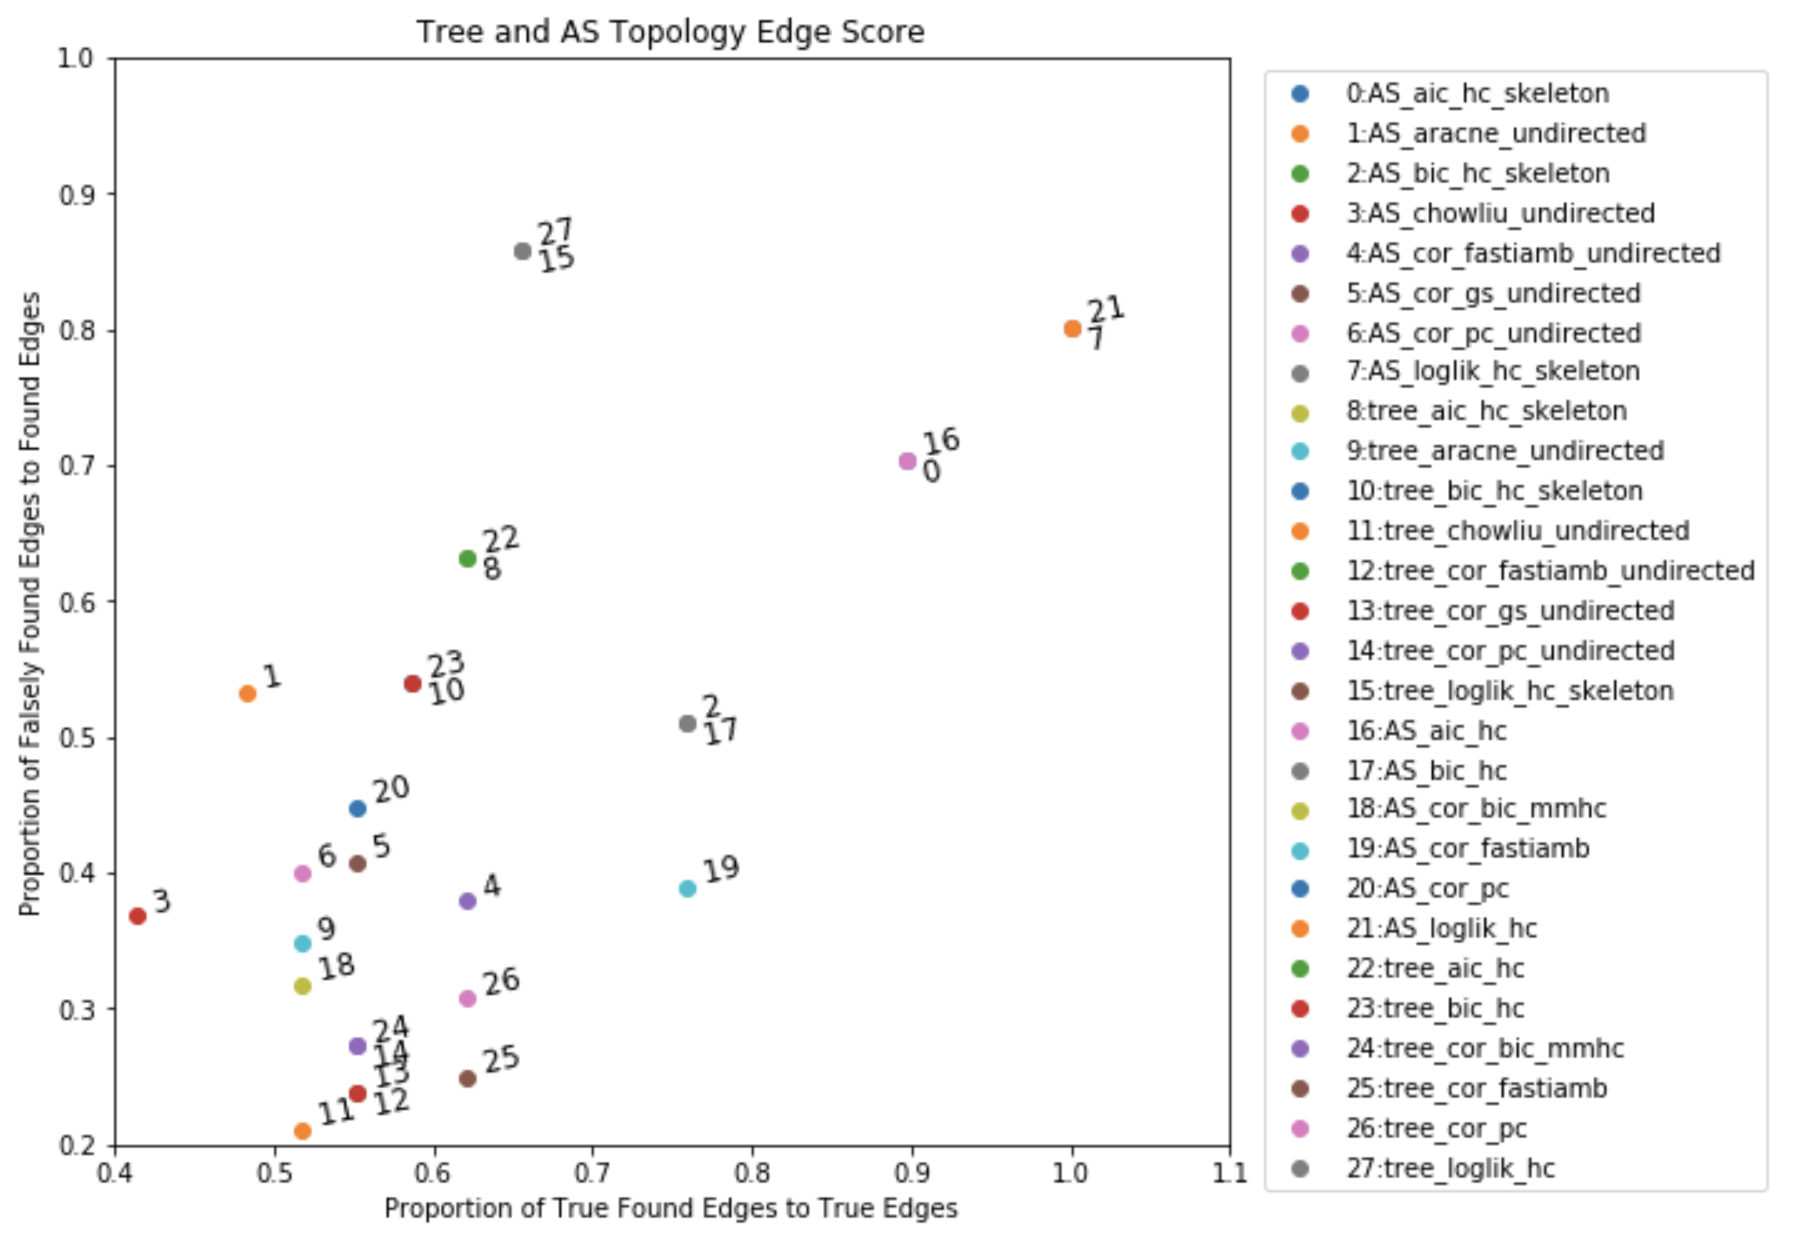
\includegraphics[height=6cm]{images/edge_scores.png}
    \caption{Scatter plot of the proportion of edges found in the learned graph that are true to the connectivity in the network relative to all possible edges in the true topology versus the proportion of edges found the learned graph that are not in the connectivity of the true topology relative to all edges in the learned graph. 
}
\label{fig:edges}
\end{figure}

\begin{figure}%
    \centering
    \subfloat{{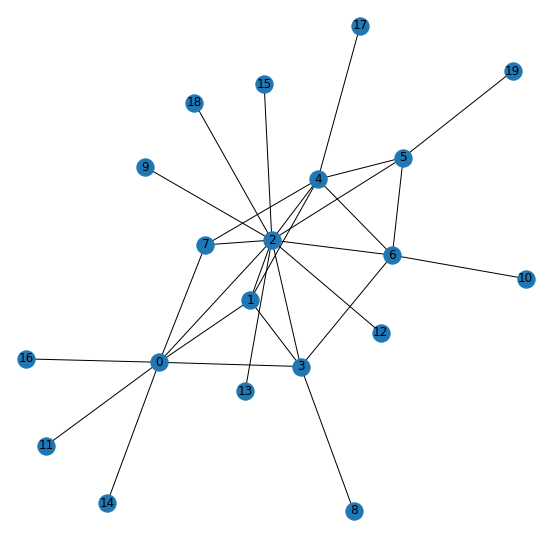
\includegraphics[width=3cm]{images/AS_graph_random_delay_200days_equalbias.png}}}
    \subfloat{{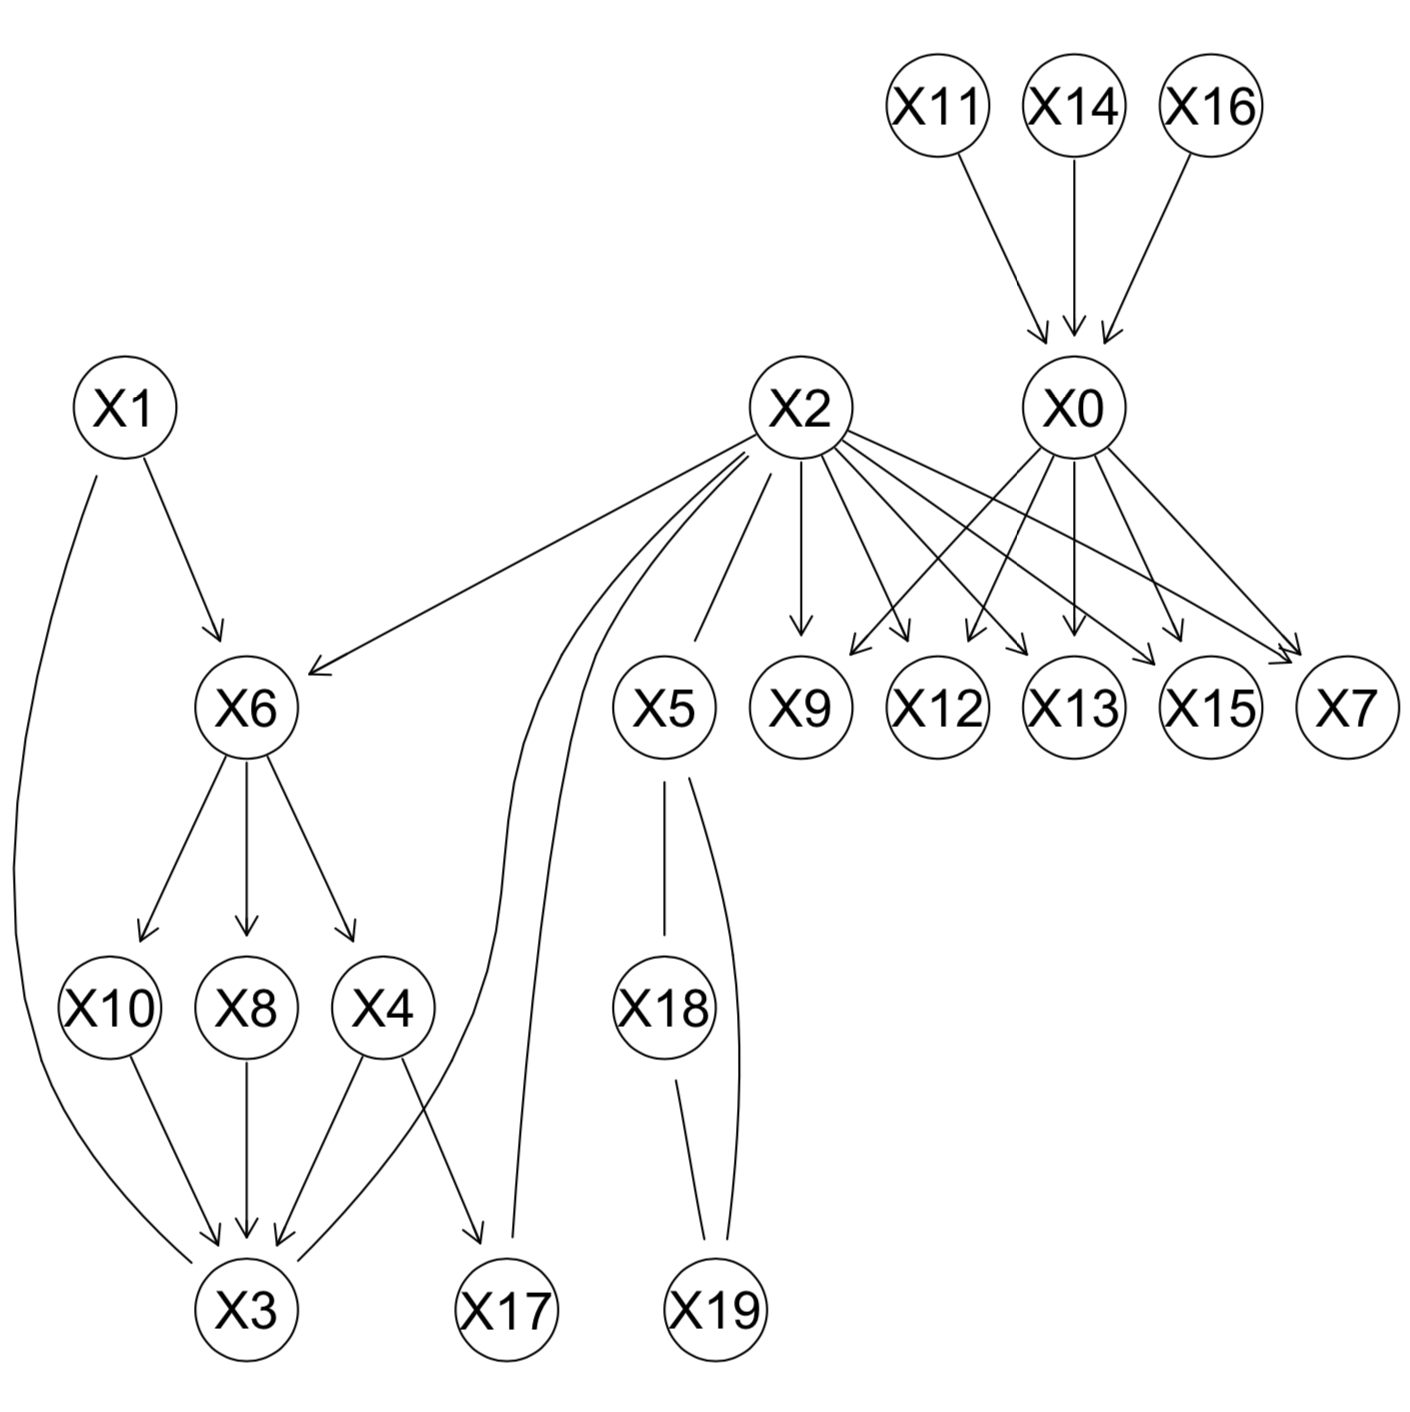
\includegraphics[width=3cm]{images/AS_fastiamb.png} }}
    \qquad
    \subfloat{{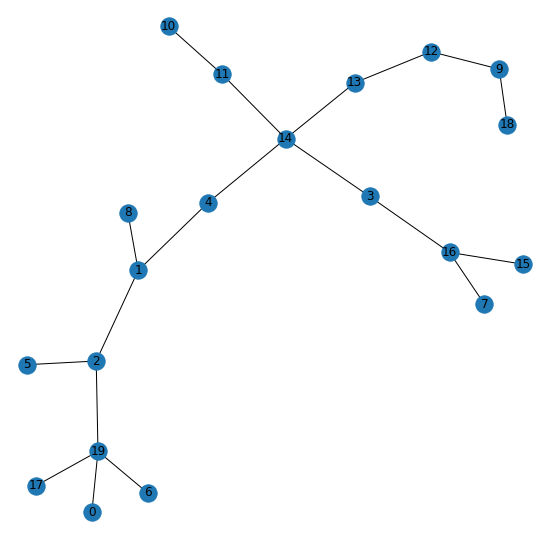
\includegraphics[width=3cm]{images/tree_graph_random_delay_200days_equalbias.png}}}
    \subfloat{{\includegraphics[width=3cm]{images/tree_fastiamb.png} }}
    \caption{Real (left-hand side) and learned (right-hand side) traffic flow connectivity for the AS (top) and tree (bottom) topologies using the fast IAMB algorithm. For the AS topology, TFT = 0.76 while FFF = 0.39. For the tree topology, TFT = 0.62 while FFF = 0.25.}
    \label{fig:graphs}

\end{figure}

It is interesting that out of the algorithms we used to learn graphical models the most accurate was the fast IAMB to learn DAGs (Figure \ref{fig:graphs}). Despite some edges being left undirected (which occurs when DAG conditional dependency statements are true when either node is the parent), most edges are directed for both topologies. We actually expected UGMs to recover more edges from the real traffic topology compared to the DAGs because any node could be a source in our simulations and therefore traffic across edges is generally bidirectional. The relative success of DAG versus UGM structure learning may have occurred since both topologies are hierarchical and thus there is effectively a topological ordering to the nodes. The nodes closer to the output nodes will have higher counts than those further away. The success of the IAMB algorithm specifically may be due to its ability to learn the Markov blanket of each node (essentially the neighborhood of the node) after performing conditional independence testing in an order determined by the mutual information of the nodes, since Markov blankets allow for fewer false positives when the neighborhood size is large (i.e., many interrelated nodes) \cite{b12}. All code for generating the simulated topologies, network traffic and DAGs as well as for comparing the learned DAGs to the real topologies is available here: \href{https://github.com/fizzX/cs143-final}{github.com/fizzX/cs143-final}.

\section{Conclusion}

DAG structure learning can be used to reveal network traffic patterns for AS and tree topologies based only on packet counts at ISP routers. To the best of our knowledge, this is the first study to compare UGM and DAG structure learning algorithms to recover network traffic flows aggregated on the host level. The project was a strong success because we showed that there is an algorithm (IAMB) that can recover far more true edges in the DAG relative to the real topology connectivity compared to extraneous edges (edges in DAG that are not shown in the real connectivity).

Our immediate next step would be to run simulations with different numbers of pings per ``day" and different numbers of ``days". This would show how robust the current findings are to sample size, which would be useful since allowing smaller sample sizes for the number of pings per ``day” would allow us to use this method to learn traffic flow patterns over shorter time intervals - useful since traffic changes over time. We would also run more simulations on different types of network topology archetypes modeled after actual content delivery networks and other types of internet service networks. This is especially important in order to evaluate whether the fast IAMB algorithm for DAG learning still succeeds for topologies that are not necessarily hierarchical. Additionally, we hope to find real-world internet traffic data for network topologies that we can observe. Although we did find real-world datasets from CAIDA along with other maps of router connectivity, we were unable to discover the actual network topology that the dataset was derived from and therefore we would have had no way to evaluate whether the learned DAG was representative of the true topology. A long-term goal would be to investigate whether other graphical models as opposed to UGMs and DAGs can be used to reveal network-wide traffic. Specifically, we could investigate how machine learning approaches such as those used for graphical neural networks could be applied to learn traffic flow patterns based only on router packet counts.

\begin{thebibliography}{00}
\bibitem{b1} Iliofotou, M., Pappu, P., Faloutsos, M., Mitzenmacher, M., Singh, S., \& Varghese, G. (2007). ``Network monitoring using traffic dispersion graphs (tdgs)''. Proceedings of the 7th ACM SIGCOMM Conference on Internet Measurement, 315-320.
\bibitem{b2} Cisco. ``Introduction to the Cisco TOP NetFlow''. May 2012.
\bibitem{b3} Donnet, B., Raoult, P., Friedman, T., \& Crovella, M. (2006). ``Deployment of an Algorithm for Large-Scale Topology Discovery". IEEE Journal on Selected Areas in Communications, 24, 2210-2220.
\bibitem{b4} Chintan, T., Mo-yuen, C., Nilsson, A., \& Trussell, H. J., (2002). ``Classification of Internet Traffic using Artificial Neural Networks''. TR-02/05 Center for Advanced Computing and Communication technical report.
\bibitem{b5} Rusek, K., Suarez-Varela, J., Mestres, A., Barlet-Ros, P., \& Cabellos-Aparicio., A. (2019). Unveiling the potential of Graph Neural Networks for network modeling and optimization in SDN. ArXiv.org, 140-151.
\bibitem{b6} Kalisch, M., Machler, M., Colombo, D., Maathuis, M. H., \& Buhlmann, P. (2012). ``Causal Inference Using Graphical Models with the R Package pcalg''. Journal of Statistical Software, 47, 1-26.
\bibitem{b7} Hausman, D., \& Woodward, J. (1999). ``Independence, invariance and the causal Markov condition''. The British Journal for the Philosophy of Science, 50, 521-583.
\bibitem{b8} White, A., \& Vignes, M. (2018). ``Causal Queries from Observational Data in Biological Systems via Bayesian Networks: An Empirical Study in Small Networks''. ArXiv.org, May 4, 2018.
\bibitem{b9} Nandy, P., Hauser, A., \& Maathuis, M. (2018). High-dimensional consistency in score-based and hybrid structure learning. Annals of Statistics, 46, 3151-3183.
\bibitem{b10} Scutari, M. (2010). Learning Bayesian Networks with the bnlearn R Package. Journal of Statistical Software, 35, 1-22.
\bibitem{b11} Spirtes, P., Glymour, C., \& Scheines, R. (2000). Causation, prediction, and search / Peter Spirtes, Clark Glymour, and Richard Scheines; with additional material by David Heckerman ... [et al.] (2nd ed., Adaptive computation and machine learning). Cambridge, Mass.: MIT Press.
\bibitem{b12} Tsamardinos, I., Aliferis, C., \& Statnikov, A. (2003). Algorithms for Large Scale Markov Blanket Discovery. Proceedings of the sixteenth international Florida artificial intelligence research society conference. 376-381.
\bibitem{b13} Scutari, M., Graafland, C., \& Gutiérrez, J. (2018). Who Learns Better Bayesian Network Structures: Accuracy and Speed of Structure Learning Algorithms. Journal of Machine Learning Research (72, Proceedings Track, PGM 2018), 416-427; extended version in International Journal of Approximate Reasoning, 115:235-253.
\bibitem{b14} Aric, A., Hagberg, D. A., \& Swart, P. J. ``Exploring network structure, dynamics, and function using NetworkX”, in Proceedings of the 7th Python in Science Conference (SciPy2008), Gäel Varoquaux, Travis Vaught, and Jarrod Millman (Eds), (Pasadena, CA USA), pp. 11–15, Aug 2008
\bibitem{b15} Elmokashfi, A., Kvalbein, A., \& Dovrolis, C. (2010). ``On the Scalability of BGP: The Role of Topology Growth.” IEEE Journal on Selected Areas in Communications, 28, 1250-1261.
\bibitem{b16} Wang, X., Lei, W., and Yingjie, W. ``An optimal algorithm for Prufer codes.” (2009). Journal of Software Engineering and Applications 2.02. 111.
\bibitem{b17} Magoni, D., \& Pansiot, J. (2001). ``Analysis of the Autonomous System network topology." Acm Sigcomm Computer Communication Review, 31, 26-37.
\bibitem{b18} R Core Team (2017). ``R: A language and environment for statistical computing". R Foundation for Statistical Computing, Vienna, Austria.
\bibitem{b19} Sekar, V., Reiter, M. K., Willinger, W., Zhang, H., Kompella, R. R., \& Anderson, D. G. (2008). ``cSAMP: A system for network-wide flow monitoring.” NSDI Proceedings of the 5th USENIX Symposium on Networked Systems Design and Implementation, 223-246.

\end{thebibliography}

\end{document}
